% (find-LATEX "2021-1-C2-somas-2-4.tex")
% (defun c () (interactive) (find-LATEXsh "lualatex -record 2021-1-C2-somas-2-4.tex" :end))
% (defun C () (interactive) (find-LATEXsh "lualatex 2021-1-C2-somas-2-4.tex" "Success!!!"))
% (defun D () (interactive) (find-pdf-page      "~/LATEX/2021-1-C2-somas-2-4.pdf"))
% (defun d () (interactive) (find-pdftools-page "~/LATEX/2021-1-C2-somas-2-4.pdf"))
% (defun e () (interactive) (find-LATEX "2021-1-C2-somas-2-4.tex"))
% (defun o () (interactive) (find-LATEX "2021-1-C2-somas-2-4.tex"))
% (defun u () (interactive) (find-latex-upload-links "2021-1-C2-somas-2-4"))
% (defun v () (interactive) (find-2a '(e) '(d)))
% (defun d0 () (interactive) (find-ebuffer "2021-1-C2-somas-2-4.pdf"))
% (defun cv () (interactive) (C) (ee-kill-this-buffer) (v) (g))
%          (code-eec-LATEX "2021-1-C2-somas-2-4")
% (find-pdf-page   "~/LATEX/2021-1-C2-somas-2-4.pdf")
% (find-sh0 "cp -v  ~/LATEX/2021-1-C2-somas-2-4.pdf /tmp/")
% (find-sh0 "cp -v  ~/LATEX/2021-1-C2-somas-2-4.pdf /tmp/pen/")
%     (find-xournalpp "/tmp/2021-1-C2-somas-2-4.pdf")
%   file:///home/edrx/LATEX/2021-1-C2-somas-2-4.pdf
%               file:///tmp/2021-1-C2-somas-2-4.pdf
%           file:///tmp/pen/2021-1-C2-somas-2-4.pdf
% http://angg.twu.net/LATEX/2021-1-C2-somas-2-4.pdf
% (find-LATEX "2019.mk")
% (find-CN-aula-links "2021-1-C2-somas-2-4" "2" "c2m211somas24" "c2so24")
%
% Video:
% (find-ssr-links "c2m211somas24" "2021-1-C2-somas-2-4")
% (code-video     "c2m211somas24video" "$S/http/angg.twu.net/eev-videos/2021-1-C2-somas-2-4.mp4")
% (find-c2m211somas24video "0:00")

% «.defs»			(to "defs")
% «.title»			(to "title")
% «.links»			(to "links")
% «.exercicio-1»		(to "exercicio-1")
%
% «.contexto»			(to "contexto")
% «.menos-de-50-tentativas»	(to "menos-de-50-tentativas")
% «.como-se-virar»		(to "como-se-virar")
% «.como-se-virar-2»		(to "como-se-virar-2")
% «.como-se-virar-3»		(to "como-se-virar-3")
% «.como-se-virar-4»		(to "como-se-virar-4")
%
% «.abusos-de-linguage»		(to "abusos-de-linguage")
% «.abusos-de-linguagem»	(to "abusos-de-linguagem")
% «.overloading-image»		(to "overloading-image")
% «.overloading-image-2»	(to "overloading-image-2")
% «.overloading-le»		(to "overloading-le")
% «.overloading-le-2»		(to "overloading-le-2")
% «.eu-amo-overloading»		(to "eu-amo-overloading")
% «.eu-amo-overloading-2»	(to "eu-amo-overloading-2")
% «.mais-sobre-bolinhas»	(to "mais-sobre-bolinhas")
% «.conjuntos-vazios»		(to "conjuntos-vazios")
%
% «.djvuize»			(to "djvuize")

\documentclass[oneside,12pt]{article}
\usepackage[colorlinks,citecolor=DarkRed,urlcolor=DarkRed]{hyperref} % (find-es "tex" "hyperref")
\usepackage{amsmath}
\usepackage{amsfonts}
\usepackage{amssymb}
\usepackage{pict2e}
\usepackage[x11names,svgnames]{xcolor} % (find-es "tex" "xcolor")
\usepackage{colorweb}                  % (find-es "tex" "colorweb")
%\usepackage{tikz}
%
% (find-dn6 "preamble6.lua" "preamble0")
%\usepackage{proof}   % For derivation trees ("%:" lines)
%\input diagxy        % For 2D diagrams ("%D" lines)
%\xyoption{curve}     % For the ".curve=" feature in 2D diagrams
%
\usepackage{edrx15}               % (find-LATEX "edrx15.sty")
\input edrxaccents.tex            % (find-LATEX "edrxaccents.tex")
\input edrxchars.tex              % (find-LATEX "edrxchars.tex")
\input edrxheadfoot.tex           % (find-LATEX "edrxheadfoot.tex")
\input edrxgac2.tex               % (find-LATEX "edrxgac2.tex")
%
%\usepackage[backend=biber,
%   style=alphabetic]{biblatex}            % (find-es "tex" "biber")
%\addbibresource{catsem-slides.bib}        % (find-LATEX "catsem-slides.bib")
%
% (find-es "tex" "geometry")
\usepackage[a6paper, landscape,
            top=1.5cm, bottom=.25cm, left=1cm, right=1cm, includefoot
           ]{geometry}
%
\begin{document}

\catcode`\^^J=10
\directlua{dofile "dednat6load.lua"}  % (find-LATEX "dednat6load.lua")

%L dofile "edrxtikz.lua"  -- (find-LATEX "edrxtikz.lua")
%L dofile "edrxpict.lua"  -- (find-LATEX "edrxpict.lua")
\pu

% «defs»  (to ".defs")
% (find-LATEX "edrx15.sty" "colors-2019")
\long\def\ColorRed   #1{{\color{Red1}#1}}
\long\def\ColorViolet#1{{\color{MagentaVioletLight}#1}}
\long\def\ColorViolet#1{{\color{Violet!50!black}#1}}
\long\def\ColorGreen #1{{\color{SpringDarkHard}#1}}
\long\def\ColorGreen #1{{\color{SpringGreenDark}#1}}
\long\def\ColorGreen #1{{\color{SpringGreen4}#1}}
\long\def\ColorGray  #1{{\color{GrayLight}#1}}
\long\def\ColorGray  #1{{\color{black!30!white}#1}}
\long\def\ColorBrown #1{{\color{Brown}#1}}
\long\def\ColorBrown #1{{\color{brown}#1}}
\long\def\ColorOrange#1{{\color{orange}#1}}

\long\def\ColorShort #1{{\color{SpringGreen4}#1}}
\long\def\ColorLong  #1{{\color{Red1}#1}}

\def\frown{\ensuremath{{=}{(}}}
\def\True {\mathbf{V}}
\def\False{\mathbf{F}}
\def\D    {\displaystyle}

\def\drafturl{http://angg.twu.net/LATEX/2021-1-C2.pdf}
\def\drafturl{http://angg.twu.net/2021.1-C2.html}
\def\draftfooter{\tiny \href{\drafturl}{\jobname{}} \ColorBrown{\shorttoday{} \hours}}

\def\V    {\mathbf{V}}
\def\F    {\mathbf{F}}
\def\ph#1 {\phantom{#1}}
\def\ph   {\phantom}



%  _____ _ _   _                               
% |_   _(_) |_| | ___   _ __   __ _  __ _  ___ 
%   | | | | __| |/ _ \ | '_ \ / _` |/ _` |/ _ \
%   | | | | |_| |  __/ | |_) | (_| | (_| |  __/
%   |_| |_|\__|_|\___| | .__/ \__,_|\__, |\___|
%                      |_|          |___/      
%
% «title»  (to ".title")
% (c2m211somas24p 1 "title")
% (c2m211somas24a   "title")

\thispagestyle{empty}

\begin{center}

\vspace*{1.2cm}

{\bf \Large Cálculo 2 - 2021.1}

\bsk

Comentários sobre o exercício 4 do

``Integrais como somas de retângulos (2)''

\bsk

Eduardo Ochs - RCN/PURO/UFF

\url{http://angg.twu.net/2021.1-C2.html}

\end{center}

\newpage

% «links»  (to ".links")
% (c2m211somas24p 2 "links")
% (c2m211somas24a   "links")

Links:

\ssk

Exercício 4 do ``somas 2'':

{\footnotesize

% (c2m211somas2p 13 "exercicio-4")
% (c2m211somas2a    "exercicio-4")
% http://angg.twu.net/LATEX/2021-1-C2-somas-2.pdf#page=13

\url{http://angg.twu.net/LATEX/2021-1-C2-somas-2.pdf\#page=13}

}


\msk

Convenção sobre como representar booleanos:

{\footnotesize

% (c2m211substp 26 "visualizando-fas-e-exs-3")
% (c2m211substa    "visualizando-fas-e-exs-3")
% http://angg.twu.net/LATEX/2021-1-C2-subst.pdf#page=26
\url{http://angg.twu.net/LATEX/2021-1-C2-subst.pdf\#page=26}

}

\bsk

\newpage

% (c2m211somas2p 8 "imagens-de-intervalos")
% (c2m211somas2a   "imagens-de-intervalos")
% (c2m211somas2p 13 "exercicio-4")
% (c2m211somas2a    "exercicio-4")


Lembre que:
%
$$\begin{array}{c}
  f(x)=
    \unitlength=10pt
    \celllower=2.5pt%
    \def\cellfont{\scriptsize}%
    %
    \vcenter{\hbox{%
    \beginpicture(0,0)(11,7)
    \pictgrid%
    \pictpiecewise{(0,3)--(3,6)--(8,1)--(11,4)}%
    \put(3,6.5){\cell{(3,6)}}%
    \put(8,0.5){\cell{(8,1)}}%
    \pictaxes%
    \end{picture}%
    }}
    =
    \scalebox{1.0}{$
    \begin{cases}
    x+3 & \text{quando $x≤3$}, \\
    9-x & \text{quando $3<x<8$}, \\
    x-7 & \text{quando $8≤x$} \\
    \end{cases}
    $}
  \\
  \\
  P(y) = (∀x∈[7,9]. \, y≤f(x))...
  \end{array}
$$

O exercício 4a pedia pra calcularmos $P(0.5)$,

mas aqui vamos discutir como calcular $P(1.5)$ ---

porque no $P(1.5)$ as figuras são mais legais.

\newpage

Vou supor que todo mundo sabe representar graficamente

subconjuntos do plano. Por exemplo:
%
$$\setofst{(x,y)∈\R^2}{x∈[1,2) \text{ e } y∈[1,2)}
  =
  % (find-latexscan-links "C2" "20210708_subconjunto_do_plano")
  % (find-xpdf-page "~/LATEX/2021-1-C2/20210708_subconjunto_do_plano.pdf")
  \myvcenter{
  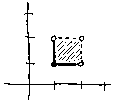
\includegraphics[height=3cm]{2021-1-C2/20210708_subconjunto_do_plano.pdf}
  }
$$

\newpage

% «exercicio-1»  (to ".exercicio-1")
% (c2m211somas24p 5 "exercicio-1")
% (c2m211somas24a   "exercicio-1")

{\bf Exercício 1.}

a) Seja $G(x,y) = (y≤f(x))$. Represente graficamente o valor

(booleano!) de $G(x,y)$ nos pontos do plano com $x∈{7,8,9}$ e

$y∈\{0,1,\ldots,7\}$, usando a convenção de que `$•$' quer dizer

``verdadeiro'' e `$∘$' quer dizer falso.

\msk

b) Represente graficamente este conjunto:
%
$$\setofst{(x,y)∈\R^2}{G(x,y)}
$$

\newpage

O modo mais rápido e mais fácil de entender de resolver o

exercício 4a é visual. Os pares $(x,y)$ que obedecem $y≤f(x)$

são exatamente os pontos deste conjunto:

% (find-latexscan-links "C2" "20210708_subconjunto_2")
% (find-xpdf-page "~/LATEX/2021-1-C2/20210708_subconjunto_2.pdf")
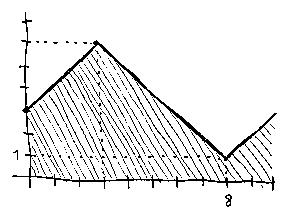
\includegraphics[height=4cm]{2021-1-C2/20210708_subconjunto_2.pdf}

E $P(1.5)$, ou seja, $(∀x∈[7,9]. \, 1.5≤f(x))$, é verdadeiro se e só se

todos os pontos do conjunto $\setofst{(x,y)∈\R^2}{y=1.5, 7≤x≤9}$

estão no conjunto dos ``pares que obedecem $y≤f(x)$''.

\newpage

Um outro modo --- equivalente ao anterior --- de calcular $P(1.5)$

é pegar todos os pontos de $\setofst{(x,y)∈\R^2}{y=1.5, 7≤x≤9}$,

e desenhar sobre cada um deles um `$•$' quando $G(x,y)$ for

verdadeiro naquele ponto e um `$∘$' quando $G(x,y)$ for falso.

\msk

A expressão
%
$$(∀x∈[7,9]. \, 1.5≤f(x))$$

vai ser verdadeira se e só se todas as (infinitas) bolinhas

que desenhamos forem pretas.

\msk

Como é difícil calcular um número infinito de expressões e

desenhar um infinito de bolinhas a gente faz só alguns casos

e tenta reconhecer o padrão.


\newpage

{\bf Exercício 2.}

Seja $f$ a função do slide 3, e:
%
$$\begin{array}{rcl}
  G(x,y) &=& (y ≤ f(x)), \\ 
    P(y) &=& (∀x∈[7,9].y ≤ f(x)) \\ 
         &=& (∀x∈[7,9].G(x,y)). \\ 
  \end{array}
$$

Desenhe num gráfico só:

a) o conjunto $\setofxyst{G(x,y)}$,

\msk

b) as (infinitas!) bolinhas brancas e pretas que

correspondem a $P(1.5)$, e faça um círculo

amassado em torno delas,

\msk

c) as (infinitas!) bolinhas brancas e pretas que

correspondem a $P(0.5)$, e faça um círculo

amassado em torno delas,

\newpage

{\bf Exercício 2 (cont.)}

\msk

d) Escreva do lado do seu gráfico algo como ``$P(1.5)$

é falso porque algumas dessas bolinhas são brancas''

e faça uma seta indo desse texto pro círculo amassado

certo.

\msk

e) Escreva do lado do seu gráfico algo como ``$P(0.5)$

é verdadeiro porque todas essas bolinhas são pretas''

e faça uma seta indo desse texto pro círculo amassado

certo.

\bsk

O desenho que você acabou de fazer serve pra mostrar

porque é que $P(1.5)$ é falso e $P(0.5)$ é verdadeiro.

Um leitor que tente entender esse desenho provavelmente

vai aprender muitas coisas -- úteis, e fáceis de generalizar --

sem muito sofrimento.


\newpage

No resto destes slides eu vou tentar explicar porque é

que o desenho que você fez no Exercício 2 é um modo

de mostrar que $P(1.5)$ é falso e $P(0.5)$ é verdadeiro

\ColorRed{MUITO melhor do que uma prova ``textual'' só por

contas e texto em português}.



\newpage

\thispagestyle{empty}

\begin{center}

\vspace*{1.2cm}

\begin{tabular}{c}
{\bf \large Parte 2:} \\
{\bf \Large Contextos} \\
\end{tabular}

\end{center}

\newpage

% «contexto»  (to ".contexto")
% (c2m211somas24p 12 "contexto")
% (c2m211somas24a    "contexto")

Quase todas as expressões matemáticas que usamos em C2

\ColorRed{dependem do contexto}. Por exemplo, a interpretação

\ColorRed{default} pra esta expressão aqui:
%
$$f(x) = x-9 = 2$$

é:
%
$$\begin{tabular}{l}
  Para toda função $f:\R→\R$ \\
  e para todo $x∈\R$ temos: \\
  $f(x) = x-9 = 2$
  \end{tabular}
$$

\bsk

Releia a dica 7:

% \ssk

{\footnotesize

% (c2m211somas1dp 7 "dica-7")
% (c2m211somas1da   "dica-7")
% http://angg.twu.net/LATEX/2021-1-C2-somas-1-dicas.pdf#page=7
\url{http://angg.twu.net/LATEX/2021-1-C2-somas-1-dicas.pdf#page=7}

}

% \ssk

Se você só escreve ``$f(x) = x-9 = 2$'' e mostra isso pro ``colega

que seja seu amigo'' ele vai levar meia hora tentando adivinhar

qual foi o contexto que você estava pensando mas não escreveu...


\newpage

% «menos-de-50-tentativas»  (to ".menos-de-50-tentativas")
% (c2m211somas24p 13 "menos-de-50-tentativas")
% (c2m211somas24a    "menos-de-50-tentativas")

...e se ele descobrir em menos de, digamos, 50 tentativas, ele

vai dizer ``ok, jóia, tá certo!''.

\msk

O ``colega que seja menos seu amigo'' vai fazer menos tentativas,

e os personagens ``o monitor'' e ``o professor'' da Dica 7 vão

checar se o que você escreveu vai ser entendido corretamente

por qualquer pessoa que saiba as convenções de como escrever

matemática.

\msk

Lembre que \ColorRed{quase todo mundo} pára de ler um texto matemático

quando vê uma besteira muito grande escrita nele. Imagine

que um ``colega que seja menos seu amigo'' te mostra a

solução dele pra um problema e te pergunta se está certa.

A solução dele começa com:
%
$$\text{Sabemos que $2=3$. Então...}$$

O que você faria?

\newpage

No slide 3 nós definimos:
%
$$\begin{array}{c}
  f(x)=
    \unitlength=10pt
    \celllower=2.5pt%
    \def\cellfont{\scriptsize}%
    %
    \vcenter{\hbox{%
    \beginpicture(0,0)(11,7)
    \pictgrid%
    \pictpiecewise{(0,3)--(3,6)--(8,1)--(11,4)}%
    \put(3,6.5){\cell{(3,6)}}%
    \put(8,0.5){\cell{(8,1)}}%
    \pictaxes%
    \end{picture}%
    }}
    =
    \scalebox{1.0}{$
    \begin{cases}
    x+3 & \text{quando $x≤3$}, \\
    9-x & \text{quando $3<x<8$}, \\
    x-7 & \text{quando $8≤x$} \\
    \end{cases}
    $}
  \\
  \\
  P(y) = (∀x∈[7,9]. \, y≤f(x))
  \end{array}
$$

Vou acrescentar mais uma definição:
%
$$
  Q(y) = (∀x∈\{7,8,9\}. \, y≤f(x))
$$

Qualquer pessoa \ColorRed{que já tenha pensado muito sobre esse problema}

sabe que $P(y)$ e $Q(y)$ são ``equivalentes''...

\newpage

...``equivalentes'' no sentido de que $P(y)$ é verdade num certo

valor de $y$ se e só se $Q(y)$ é verdade naquele mesmo $y$.

Isto pode ser escrito em linguagem matemática deste jeito:
%
$$∀y∈\R. (P(y) ↔ Q(y))$$

Dá pra demonstrar que `$∀y∈\R. (P(y) ↔ Q(y))$' é verdade

\ColorRed{pra função $f$ que estamos usando}. A demonstração formal

disso é difícil, e se você está interessado em aprender como

fazer ela você pode entrar num grupo de Telegram que eu

vou criar pra gente discutir isso \ColorRed{mas no qual eu só vou

deixar entrar quem já aprendeu sups e infs}.

\newpage

Se na sua demonstração você disser --

explicitamente ou implicitamente --

que é óbvio que isto aqui
%
$$∀y∈\R. (P(y) ↔ Q(y))$$

é verdade \ColorRed{quase qualquer pessoa} vai parar de ler

nesse ponto, e vai dizer:
%
$$\text{\Large \bf NÃO É ÓBVIO NÃO!!!}$$

E ela vai ter razão.


\newpage

% «como-se-virar»  (to ".como-se-virar")
% (c2m211somas24p 17 "como-se-virar")
% (c2m211somas24a    "como-se-virar")

{\bf Como se virar sem demonstrações formais?}

Se você reler os exercícios que eu passei você vai ver que

quase todos começam com ``calcule'' ou com ``represente

graficamente''; uns poucos deles dizem ``expanda'' ou

``calcule passo a passo''.

\msk

Nos exercícios de ``calcule'' basta você conseguir

chegar ao resultado certo por um raciocínio que faça

sentido pra você. Se você puder discutir com colegas,

explicar o seu raciocínio pra eles e chegar a uma

explicação que faça sentido pro ``colega que seja

seu amigo'' da Dica 7, ótimo. Não é necessário chegar

a uma demonstração que faça sentido pra alguém que

vá ser super rigoroso e que vá parar assim que

encontrar o primeiro erro.

\newpage

% «como-se-virar-2»  (to ".como-se-virar-2")
% (c2m211somas24p 18 "como-se-virar-2")
% (c2m211somas24a    "como-se-virar-2")

{\bf Como se virar sem demonstrações formais? (2)}

Dá pra gente apresentar argumentos informais pra

pessoas rigorosíssimas de um jeito que elas aceitem,

sim -- DESDE QUE A GENTE MARQUE CLARAMENTE

AS PARTES QUE NÃO ESTÃO TOTALMENTE FORMAIS.

\msk

Por exemplo, se você escrever algo como ``Rascunho'',

``Esboço'', ou ``Não sei escrever isso aqui direito!!!''

em cima destas contas,
%
$$\begin{array}{ll}
  P(0.5) \\
  f(7) = 9-x = 2 & \V \\ 
  f(8) = x-7 = 1 & \V \\ 
  f(9) = x-7 = 2 & \V \\ 
  P(0.5) \;\;\; \V \\
  \end{array}
$$

o leitor não vai achar que tem erros (graves) aí.

\newpage

% «como-se-virar-3»  (to ".como-se-virar-3")
% (c2m211somas24p 19 "como-se-virar-3")
% (c2m211somas24a    "como-se-virar-3")

{\bf Como se virar sem demonstrações formais? (3)}

E se você mostrar essas contas
%
$$\begin{array}{ll}
  P(0.5) \\
  f(7) = 9-x = 2 & \V \\ 
  f(8) = x-7 = 1 & \V \\ 
  f(9) = x-7 = 2 & \V \\ 
  P(0.5) \;\;\; \V \\
  \end{array}
$$

no tal grupo do Telegram que é só pra quem já

aprendeu sups e infs e perguntar algo como:

``gente, vocês conseguem entender isso aqui?

Como a gente escreve isso de um jeito formal?''

aí as pessoas vão discutir como escrever os contextos

que faltam, como reescrever o espaço antes de cada `$\V$'

de um jeito que todo mundo entenda, etc...

\newpage

% «como-se-virar-4»  (to ".como-se-virar-4")
% (c2m211somas24p 20 "como-se-virar-4")
% (c2m211somas24a    "como-se-virar-4")

{\bf Como se virar sem demonstrações formais? (4)}

Repare que a pergunta ``isso aqui tá certo?''
%
$$\begin{array}{ll}
  P(0.5) \\
  f(7) = 9-x = 2 & \V \\ 
  f(8) = x-7 = 1 & \V \\ 
  f(9) = x-7 = 2 & \V \\ 
  P(0.5) \;\;\; \V \\
  \end{array}
$$

é totalmente diferente da pergunta:

\ssk

``gente, vocês conseguem entender isso aqui?

Como a gente escreve isso de um jeito formal?''

\msk

...e eu considero que a gente não deve discutir a segunda

pergunta nos grupos ``normais'' das duas turmas enquanto

ainda tem muita gente que ainda não aprendeu a visualizar

sups, infs, e a definição de integral.

\newpage

%   ___                 _                 _ _             
%  / _ \__   _____ _ __| | ___   __ _  __| (_)_ __   __ _ 
% | | | \ \ / / _ \ '__| |/ _ \ / _` |/ _` | | '_ \ / _` |
% | |_| |\ V /  __/ |  | | (_) | (_| | (_| | | | | | (_| |
%  \___/  \_/ \___|_|  |_|\___/ \__,_|\__,_|_|_| |_|\__, |
%                                                   |___/ 

\thispagestyle{empty}

\begin{center}

\vspace*{1.2cm}

\begin{tabular}{c}
{\bf \large Parte 3:} \\
{\bf \Large Abusos de linguagem} \\
{\bf \Large e overloading} \\
\end{tabular}

\end{center}

\newpage

% «abusos-de-linguagem»  (to ".abusos-de-linguagem")
% (c2m211somas24p 22 "abusos-de-linguagem")
% (c2m211somas24a    "abusos-de-linguagem")

{\bf Abusos de linguagem}

Tem expressões que se a gente usar \ColorRed{entre aspas}

quase todo mundo vai entender... por exemplo:

\begin{quotation}

  Para todo ponto $(x,y)$ no ``intervalo fechado''

  indo do ponto $(7,1)$ ao ponto $(9,1)$ a proposição

  $G(x,y)$ é verdadeira.

\end{quotation}

Um dos tipos mais comuns de abuso de linguagem

é o \ColorRed{overloading} --- mas sem uma definição explícita

de como a operação funciona no tipo novo.

Um exemplo (famoso) de overloading:

$$2 + 3 = 5
  \qquad
  \pmat{2 \\ 20} + \pmat{3 \\ 300} = \pmat{5 \\ 320}
  \qquad
  \qquad
$$

\newpage

% «overloading-image»  (to ".overloading-image")
% (c2m211somas24p 23 "overloading-image")
% (c2m211somas24a    "overloading-image")

{\bf Exemplo de overloading: imagens de conjuntos}

Lembre que a partir de uma função $f:\R→\R$ qualquer

nós definimos uma função $F$ que recebe subconjuntos

de $\R$ e retorna subconjuntos de $\R$...
%
$$F(\{7,8,9\}) = \{f(7), f(8), f(9)\} = \{2, 1, 2\}$$

Alguns livros usam a \ColorRed{mesma notação} pra $f$ e $F$:
%
$$f(\{7,8,9\}) = \{f(7), f(8), f(9)\} = \{2, 1, 2\}$$

e aí pra decidir qual é o significado de $f$

a gente precisa descobrir o tipo do argumento

dela -- se é número ou conjunto de números. 

\newpage

% «overloading-image-2»  (to ".overloading-image-2")
% (c2m211somas24p 24 "overloading-image-2")
% (c2m211somas24a    "overloading-image-2")

{\bf Exemplo de overloading: imagens de conjuntos (2)}

Estes livros \ColorRed{estendem} o significado original da $f$ assim:
%
$$\begin{array}{l}
  \text{Se $A⊂\R$ então:} \\
  $f(A) = \setofst{f(a)}{a∈A}$ \\
  \end{array}
$$

Eu estou evitando esse tipo de overloading no curso porque

acho que ele deixaria muitos alunos meio desesperados...

Só que várias pessoas tentaram inventar os seus próprios

jeitos de fazer overloading... por exemplo:
%
$$\{2,3,4\} ≤ \{3,4,5\}$$

Isso é muito ambíguo -- eu consigo pensar em vários

jeitos de definir esse `$≤$' em conjuntos...

\newpage

% «overloading-le»  (to ".overloading-le")
% (c2m211somas24p 25 "overloading-le")
% (c2m211somas24a    "overloading-le")

{\bf Exemplo de overloading ambíguo: `$≤$' em conjuntos}

Se usarmos esta definição pro `$≤$' em conjuntos,
%
$$\begin{array}{l}
  \text{Se $A,B⊂\R$ então:} \\
  (A≤B) = (∀a∈A.∀b∈B.a≤b) \\
  \end{array}
$$

então temos $(\{2,3,4\} ≤ \{3,4,5\}) = \F$.

\bsk

Se usarmos esta definição pro `$≤$' em conjuntos,
%
$$\begin{array}{l}
  \text{Se $A,B⊂\R$ então:} \\
  (A≤B) = (∀a∈A.∃b∈B.a≤b) \\
  \end{array}
$$

então temos $(\{2,3,4\} ≤ \{3,4,5\}) = \V$.

\newpage

% «overloading-le-2»  (to ".overloading-le-2")
% (c2m211somas24p 26 "overloading-le-2")
% (c2m211somas24a    "overloading-le-2")

{\bf Exemplo de overloading ambíguo: `$≤$' em conjuntos (2)}

...e se usarmos esta outra definição pro `$≤$' em conjuntos,
%
$$\begin{array}{l}
  \text{Se $A,B⊂\R$ então:} \\
  (A≤B) = \setofst{a∈A}{∀b∈B.a≤b} \\
  \end{array}
$$

então temos $(\{2,3,4\} ≤ \{3,4,5\}) = \{2,3\}$.

\bsk

$\frown$


\newpage

% «eu-amo-overloading»  (to ".eu-amo-overloading")
% (c2m211somas24p 27 "eu-amo-overloading")
% (c2m211somas24a    "eu-amo-overloading")

{\bf ``Eu amo overloading! E agora?''}

\msk

Algumas pessoas:

1) adoram usar overloadings nas suas contas informais,

2) querem aprender a formalizar essas contas.

O que elas podem fazer?

\msk

Respostas:

a) Avisar que aquelas contas são informais

b) traduzir os overloadings pra algo formal -- como:
%
$$\begin{array}{l}
  \{2,3,4\} ≤ \{3,4,5\} \\[2.5pt]
  \squigto \;\; ∀a∈\{2,3,4\}.∀b∈\{3,4,5\}.a≤b \\
  \end{array}
$$

c) aprender a \ColorRed{definir overloadings formalmente}.

\msk

Aparentemente o (c) é o mais legal de todos, né?...


\newpage

% «eu-amo-overloading-2»  (to ".eu-amo-overloading-2")
% (c2m211somas24p 28 "eu-amo-overloading-2")
% (c2m211somas24a    "eu-amo-overloading-2")

{\bf ``Eu amo overloading! E agora?'' (2)}

\msk

...só que pra

\ssk

\ColorRed{c) aprender a definir overloadings formalmente}

\ssk

você vai ter que aprender a testar as suas definições --

e pra isso você vai ter que aprender o (b):

\ssk

\ColorRed{b) traduzir os overloadings pra algo formal}

\ssk

e você vai ter que testar as suas traduções em um

monte de casos. A gente só consegue aprender o (c)

depois de já ter virado faixa-preta em usar o `$∀$', o `$∃$',

o `$\setofst{}{}$', e em tipar e em calcular expressões,

e em fazer definições mais simples e testar elas...

\msk

Então você vai ter que começar aprendendo o (a) e o (b).

\msk

$\frown$


\newpage

% «mais-sobre-bolinhas»  (to ".mais-sobre-bolinhas")
% (c2m211somas24p 29 "mais-sobre-bolinhas")
% (c2m211somas24a    "mais-sobre-bolinhas")

\thispagestyle{empty}

\begin{center}

\vspace*{1.2cm}

\begin{tabular}{c}
{\bf \large Parte 4:} \\
{\bf \Large Mais sobre bolinhas} \\
\end{tabular}

\end{center}

\newpage

Lembre que estamos tentando aprender a calcular

expressões como estas \ColorRed{visualmente}, por bolinhas...
%
$$\begin{array}{l}
  ∀x∈\{1,2,3\}.x^2>4 \\
  ∃x∈\{1,2,3\}.x^2>4 \\
  \setofst{x∈\{1,2,3\}}{x^2>4} \\
  \end{array}
  \qquad
  \begin{array}{l}
  ∀x∈[1,3].x^2>4 \\
  ∃x∈[1,3].x^2>4 \\
  \setofst{x∈[1,3]}{x^2>4} \\
  \end{array}
$$

...porque não vai dar tempo de todo mundo aprender a

calculá-las via demonstrações formais. Então todo mundo

vai ter que aprender os métodos visuais \ColorRed{primeiro}, e quem

conseguir aprendê-los pode vir discutir demonstrações

formais num outro grupo do Telegram.

\newpage

Lembre também que se você calcular coisas via bolinhas

em cursos de outros professores eles podem não entender

e podem ficar putos. Considere que o método das bolinhas

é principalmente pra você aprender a calcular certas coisas

\ColorRed{de cabeça} -- ou em rascunhos no canto do papel.

\newpage

Lembre que pra calcular estas expressões

$$\begin{array}{l}
  ∀x∈\{1,2,3\}.x^2>4 \\
  ∃x∈\{1,2,3\}.x^2>4 \\
  \setofst{x∈\{1,2,3\}}{x^2>4} \\
  \end{array}
$$

nós podemos \ColorRed{começar} representando os resultados

da expressão $x^2>4$ nos três valores de $x$ que são

``gerados'' pelo $x∈\{1,2,3\}$...
%
$$\begin{array}{c}
    \unitlength=20pt
    \celllower=2.5pt%
    \def\cellfont{\scriptsize}%
    %
    \vcenter{\hbox{%
      \beginpicture(-1,-1)(4,1)
      \pictgrid%
      \pictpiecewise{(1,0)o (2,0)o (3,0)c}%
      \pictaxes%
      \end{picture}%
    }}
  \end{array}
$$


Lembre que a gente viu ``geradores'' e ``filtros'' aqui:

\ssk

{\footnotesize

% (mpgp 8 "comprehension")
% (mpga   "comprehension")
% http://angg.twu.net/LATEX/material-para-GA.pdf#page=8
\url{http://angg.twu.net/LATEX/material-para-GA.pdf#page=8}

}

\newpage

A expressão
%
$$∀x∈\{1,2,3\}.x^2>4$$

é \ColorRed{verdadeira se e só se todas} as bolinhas são pretas.

A expressão
%
$$∃x∈\{1,2,3\}.x^2>4$$

é \ColorRed{verdadeira se e só se alguma} bolinha é preta.

E o resultado de
%
$$\setofst{x∈\{1,2,3\}}{x^2>4}$$

é o \ColorRed{conjunto} de todos os `$x$'zes cujas bolinhas são pretas:

$$\setofst{x∈\{1,2,3\}}{x^2>4} = \{3\}.$$

\newpage

{\bf E pra conjuntos infinitos?}

Pra conjuntos infinitos --- como o intervalo $[1,3]$ ---

nós podemos fazer algo parecido, mas vamos ter

que fazer um desenho que \ColorRed{finja} que tem infinitas

bolinhas... por exemplo:

$$\begin{array}{c}
    \unitlength=25pt
    \celllower=2.5pt%
    \def\cellfont{\scriptsize}%
    %
    \vcenter{\hbox{%
      \beginpicture(-1,-1)(4,1)
      \pictgrid%
      \pictpiecewise{(1.0,0)o (1.2,0)o (1.4,0)o (1.6,0)o (1.8,0)o
                     (2.0,0)o (2.2,0)c (2.4,0)c (2.6,0)c (2.8,0)c
                     (3.0,0)c}%
      \pictaxes%
      \end{picture}%
    }}
  \end{array}
$$

Se fizermos um desenho razoável um leitor com uma certa

boa vontade vai conseguir entender que temos bolinhas

brancas em $x∈[1,2]$ e bolinhas pretas em $x∈(2,3]$...

\bsk

...e aí $\setofst{x∈[1,3]}{x^2>4} = (2,3]$. \quad \smile


\newpage

% «conjuntos-vazios»  (to ".conjuntos-vazios")
% (c2m211somas24p 35 "conjuntos-vazios")
% (c2m211somas24a    "conjuntos-vazios")

{\bf E pra conjuntos vazios?}

Você lembra porque a gente define que $2^0=1$?

É porque o 1 é o elemento neutro da multiplicação,

e aí a gente tem:
%
$$\begin{array}{rclcl}
  2^3·2^2 &=& (2·2·2)·(2·2)   &=& 2^5 \\
  2^4·2^1 &=& (2·2·2·2)·(2)   &=& 2^5 \\
  2^5·2^0 &=& (2·2·2·2·2)·2^0 \\
          &=& (2·2·2·2·2)·1 \\
          &=& (2·2·2·2·2)     &=& 2^5 \\
  \end{array}
$$

A gente vai ter algo assim

pro `$∀$' e pro `$∃$' também:

$(∀x∈∅.P(x)) = \V$ \;\; (porque $\V$ é o elemento neutro do $∧$) 

$(∃x∈∅.P(x)) = \F$ \;\;\, (porque $\F$ é o elemento neutro do $∨$)

\newpage

{\bf E pra conjuntos vazios? (2)}

Veja:
%
\def\myfa#1{(∀x∈\{#1\}.P(x))}
\def\myex#1{(∃x∈\{#1\}.P(x))}
\def\myfae {(∀x∈∅.P(x))}
\def\myexe {(∃x∈∅.P(x))}
%
$$\scalebox{0.8}{$
  \begin{array}{rcl}
  \myfa{2,4} ∧ \myfa{9,20} &=& (P(2)∧P(4))∧(P(9)∧P(20)) \\
  \myfa{2,4,9} ∧ \myfa{20} &=& (P(2)∧P(4)∧P(9))∧(P(20)) \\
  \myfa{2,4,9,20} ∧ \myfae &=& (P(2)∧P(4)∧P(9)∧P(20))∧\V \\
                           &=& (P(2)∧P(4)∧P(9)∧P(20)) \\
  \\
  \myex{2,4} ∨ \myex{9,20} &=& (P(2)∨P(4))∨(P(9)∨P(20)) \\
  \myex{2,4,9} ∨ \myex{20} &=& (P(2)∨P(4)∨P(9))∨(P(20)) \\
  \myex{2,4,9,20} ∨ \myexe &=& (P(2)∨P(4)∨P(9)∨P(20))∨\F \\
                           &=& (P(2)∨P(4)∨P(9)∨P(20)) \\
  \end{array}
  $}
$$


\newpage

\phantom{a}

%\printbibliography

\GenericWarning{Success:}{Success!!!}  % Used by `M-x cv'

\end{document}

%  ____  _             _         
% |  _ \(_)_   ___   _(_)_______ 
% | | | | \ \ / / | | | |_  / _ \
% | |_| | |\ V /| |_| | |/ /  __/
% |____// | \_/  \__,_|_/___\___|
%     |__/                       
%
% «djvuize»  (to ".djvuize")
% (find-LATEXgrep "grep --color -nH --null -e djvuize 2020-1*.tex")

 (eepitch-shell)
 (eepitch-kill)
 (eepitch-shell)
# (find-fline "~/2021.1-C2/")
# (find-fline "~/LATEX/2021-1-C2/")
# (find-fline "~/bin/djvuize")

cd /tmp/
for i in *.jpg; do echo f $(basename $i .jpg); done

f () { rm -fv $1.png $1.pdf; djvuize $1.pdf }
f () { rm -fv $1.png $1.pdf; djvuize WHITEBOARDOPTS="-m 1.0" $1.pdf; xpdf $1.pdf }
f () { rm -fv $1.png $1.pdf; djvuize WHITEBOARDOPTS="-m 0.5" $1.pdf; xpdf $1.pdf }
f () { rm -fv $1.png $1.pdf; djvuize WHITEBOARDOPTS="-m 0.25" $1.pdf; xpdf $1.pdf }
f () { rm -fv $1.png $1.pdf; djvuize WHITEBOARDOPTS="-m 0.125" $1.pdf; xpdf $1.pdf }
f () { cp -fv $1.png $1.pdf       ~/2021.1-C2/
       cp -fv        $1.pdf ~/LATEX/2021-1-C2/
       cat <<%%%
% (find-latexscan-links "C2" "$1")
%%%
}

f 20210708_subconjunto_2
f 20210708_subconjunto_do_plano

f 20201213_area_em_funcao_de_theta
f 20201213_area_em_funcao_de_x
f 20201213_area_fatias_pizza



%  __  __       _        
% |  \/  | __ _| | _____ 
% | |\/| |/ _` | |/ / _ \
% | |  | | (_| |   <  __/
% |_|  |_|\__,_|_|\_\___|
%                        
% <make>

 (eepitch-shell)
 (eepitch-kill)
 (eepitch-shell)
# (find-LATEXfile "2019planar-has-1.mk")
make -f 2019.mk STEM=2021-1-C2-somas-2-4 veryclean
make -f 2019.mk STEM=2021-1-C2-somas-2-4 pdf

% Local Variables:
% coding: utf-8-unix
% ee-tla: "c2so24"
% ee-tla: "c2m211somas24"
% End:
